% vim:encoding=utf8 ft=tex sts=2 sw=2 et:

\documentclass{classrep}
\usepackage[utf8]{inputenc}
\usepackage[a4paper, margin=1in]{geometry}
\usepackage{graphicx}

\studycycle{Matematyka, studia dzienne, mag II st.}
\coursesemester{II}

%\coursename{Angelologia teoretyczna i stosowana}
\coursename{Eksploracja Danych w Javie}
\courseyear{2016/2017}

\courseteacher{dr. Andrzejczak}
\coursegroup{poniedziałek 12:15}

\author{
  \studentinfo{Norbert Landrat}{213518} \and
  \studentinfo{Adrian Grzelak}{213506}
}

\title{Rozpoznawanie podrabianych banknotów}

\begin{document}

\maketitle

\section{Cel projektu}
Projekt polegał na nauce rozpoznawania czy badany banknot jest prawdziwy używając dostępnej bazy danych opisaną w rozdziale 2. Baza zawiera 1372 wpisy z których każdy należy do jednego z 2 rodzajów banknotów (prawdziwy i sfałszowany). Wejściem jest pięć parametrów rzeczywistych, a jako wyjście oczekiwano odpowiedzi, czy badany banknot jest sfałszowany. Przeprowadzono badanie, które miało określić, jaka metoda najlepiej rozwiąże ten problem. Pierwsza metoda użyta do badania dostępnej bazy danych to perceptron wielowarstwowy. Następnie wykorzystano klasyfikator SVM. Obie metody zostały szczegółowo opisane w rozdziałach 3 i 4.

\section{Opis danych}
Rozdział ten będzie poświęcony szczegółowemu opisowi danych, które zostaną poddane klasyfikacji. Dane zostały pobrane z repozytorium UCI (https://archive.ics.uci.edu/ml/datasets/banknote+authentication). Autorem powyższych danych jest Volke Lohweg (University of Applied Sciences, Ostwestfalen-Lippe, volker.lohweg '@' hs-owl.de), a donatorem Helene Doerksen (University of Applied Sciences, Ostwestfalen-Lippe, helene.doerksen '@' hs-owl.de). Pochodzą z sierpnia 2012 r.

Dane zostały wydobyte ze zdjęć, które zostały zrobione prawdziwym i sfałszowanym banknotom. W celu transformacji danych na postać cyfrową została użyta kamera przemysłowa, która jest najczęściej używana przy inspekcji wydruku banknotów. Zdjęcia mają wymiary 400 x 400 pikseli. Z powodów technicznych (obiektyw kamery, odległość od badanych przedmiotów) zdjęcia zostały robione w odcieniu szarości  o rozdzielczości 660 dpi. Aby uzyskać konkretne cechy ze zdjęć została użyta transformata falkowa. 

Informacje o atrybutach
\begin{enumerate}
\item wariancja zdjęcia po przekształceniu transformatą falkową
\item skośność zdjęcia po przekształceniu transformatą falkową
\item kurtoza zdjęcia po przekształceniu transformatą falkową
\item entropia zdjęcia
\item klasa
\end{enumerate}
Liczba instancji: 1372

Szczegółowe informacje dotyczące poszczególnych cech
\begin{enumerate}
\item wariancja - wartości numeryczne
\begin{center}
	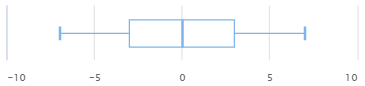
\includegraphics[height=2cm]{wariancja.png}
\end{center}
\item skośność - wartości numeryczne
\begin{center}
	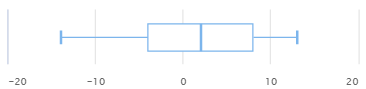
\includegraphics[height=2cm]{skosnosc.png}
\end{center}
\item kurtoza - wartości numeryczne
\begin{center}
	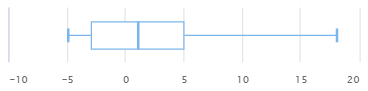
\includegraphics[height=2cm]{kurtoza.png}
\end{center}
\item entropia - wartości numeryczne
\begin{center}
	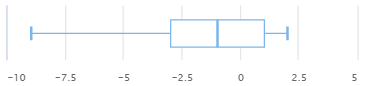
\includegraphics[height=2cm]{entropia.png}
\end{center}
\item klasa – dwie wartości (1 – banknot prawdziwy, 2 – banknot sfałszowany)
\end{enumerate}


\section{Perceptron wielowarstwowy}

Perceptron wielowarstwowy – prosta sieć neuronowa składająca się z co najmniej dwóch neuronów McCullocha-Pittsa ułożonych warstwowo, implementująca algorytm uczenia nadzorowanego klasyfikatorów binarnych. Perceptron wielowarstwowy jest funkcją, która potrafi określić przynależność parametrów wejściowych do jednej z dwóch klas. W przeciwieństwie do perceptronu jednowarstwowego może być wykorzystywany do klasyfikowania zbiorów, które nie są liniowo separowalne.

\begin{center}
	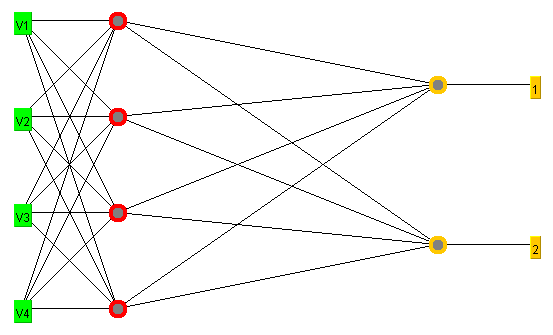
\includegraphics[height=8cm]{siec.png}
	
	
	\textbf{Rysunek 1.} Otrzymana sieć neuronowa
\end{center}

Dla celów naszego eksperymentu stowrzyliśmy sieć z 4 neuronami w warstwie ukrytej, przyjęliśmy współczynnik momentum 0.2, Współczynnik nauki 0.3. I ustawiliśmy czas uczenia się zbioru na 800 epok. W trakcie procesu uczenia 10\% elementow stanowilo zbior walidacyjny.

Perceptron w tak zdefiniowanym procesie zdołał się nauczyć rozpoznawać elementy ze 100\% skutecznością!

\section{Klasyfikator leniwy k – najbliższych sąsiadów}
\subsection{Algorytm k-NN}
Ustalamy wartość k (najlepiej liczbę nieparzystą, zwykle ok. 5-15).
Dla każdego obiektu testowego o*:
\begin{enumerate}
\item wyznaczamy odległość r(o*,x) pomiędzy o* i każdym obiektem treningowym x
\item znajdujemy k obiektów treningowych najbliższych o*
\item wśród wartości decyzji odpowiadających tym obiektom wykonujemy głosowanie
\item najczęściej występującą wartość decyzji przypisujemy obiektowi o*
\end{enumerate}
\subsection{Uwagi techniczne}
Parametr k możemy dobrać eksperymentalnie. Licząc na próbce testowej wyniki dla pewnego k, otrzymujemy przy okazji wyniki dla wszystkich wartości mniejszych.
Czas uczenia (w wersji podstawowej algorytmu) jest bardzo krótki, gdyż nauka polega na zapamiętaniu całej próbki treningowej. Łatwo stosować metodę leave-one-out.
Klasyfikacja nowych przypadków jest dosyć powolna. Sposoby na przyspieszenie:
\begin{enumerate}
\item selekcja obiektów – wybór pewnego podzbioru dającego zbliżone wyniki klasyfikacji
\item podział zbioru obiektów na podzbiory i przeszukiwanie tylko niektórych z nich.
\end{enumerate}

W przypadku badania klasyfikatorem kNN kroswalidacja dzielona na 10 podzbiorów tylko w jednym przypadku daje 100% skuteczności. Staje się to przy użyciu metryki filtrowanej z parametrami: dystans – Euklidesowy i filtrem korzystającym z 10 atrybutów, 42 nasion i rozkładzie – Sparse1. W zdecydowanej większości przypadków skuteczność metody była na poziomie 99,85%. Działo się tak w przypadku doboru sąsiadów od 1 do 11 oraz przy różnych metrykach – zaczynając od najprostszej – Euklidesowej, poprzez Minkowskiego, Manhattan kończąc na metryce Czebyszeva.  


\section{Wnioski z badania}
Analizowany zbiór jest bardzo trafnie dobrany do celów klasyfikowania. Dane w przypadku obu metod są klasyfikowane z wysoką skutecznością (dochodząc nawet do 100\%), co może oznaczać, że metoda sprawdzania sfałszowanych banknotów może znaleźć odzwierciedlenie w rzeczywistości. W metodzie k – najbliższych sąsiadów zauważalny jest wpływ liczby sąsiadów na skuteczność kroswalidacji. Począwszy od 11 sąsiadów wraz ze wzrostem parametru skuteczność sklasyfikowanych instancji maleje. W procesie nauczania perceptronu z kolei duży wpływ na osiągane wyniki ma ilość neuronów w wartswie ukrytej. Zbyt mała ich ilość może doprowadzić do słabego nauczenia się wzorca, natomiast zbyt duża do zjawiska przeuczenia (Perceptron doskonale rozpoznaje elementy ze zbioru nauczającego, ale natrafia na problemy przy danych pochodzących spoza tego zbioru.



\end{document}
